\chapter{Results: Imaging}
\label{chapter:imaging}

%\emph{\color{red}do corr. on p-meter sensitive A ($\times$1.57) and 89 percent optical flat T}

Results presented in Chapter \ref{chapter:spectroscopy} demonstrate the best conditions for imaging small numbers of Ba atoms in SXe.  Optimum excitation wavelengths were determined by studying the excitation spectra of the signal as well as the background.  Bleaching studies determined optimum laser intensities to be used.  Deposits made at $50 \pm 5$~K produced more Ba fluorescence signal than those made at 11~K.  An image of Ba atoms emitting at 577 and 591~nm is presented in Sec. \ref{sec:imaging590and577} at the level of $\leq 2.7 \times 10^{3}$ average atoms exposed. Images of Ba\ atoms emitting at 619~nm are presented down to the single-atom level in Sec. \ref{sec:imaging619}.  Initial scanned images of Ba\textsuperscript{+} deposits are presented in Sec. \ref{sec:scanning}.

Though the imaging spectrometer can produce spacial images with the 0-order grating reflection, better collection efficiency and imaging quality are achieved by removing the spectrometer and imaging directly onto the CCD.  Band-pass filters were used to pass the desired Ba fluorescence peak(s) while attenuating laser scatter and sapphire fluorescence.

%angle=90,
\begin{figure} %[H]
        \centering
                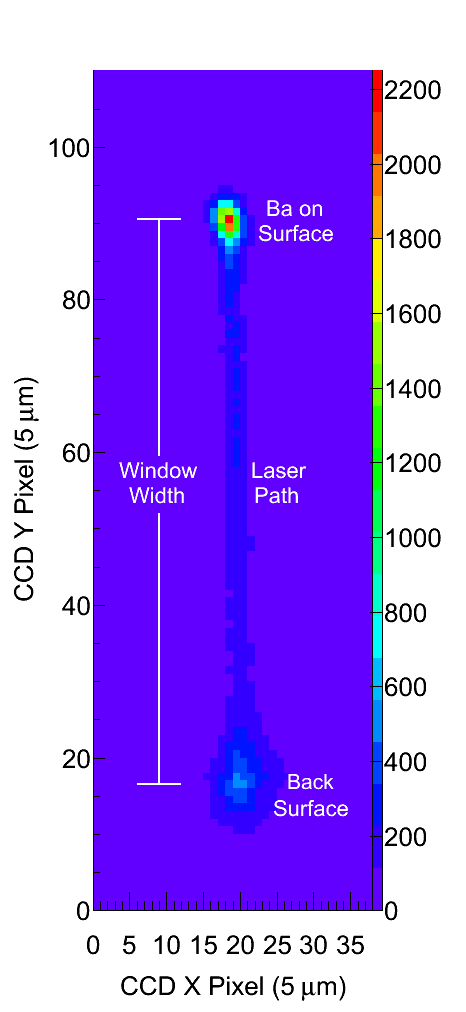
\includegraphics[width=.4\textwidth]{figures/imageExamp.png}
                \caption{Example image of focused laser exciting a Ba\textsuperscript{+} deposit on a c-plane sapphire window of 0.5~mm thickness.  Fluorescence is passed by 620-nm band-pass filter.}
\label{fig:imageexamp}
\end{figure}

An example image of the focused 570~nm dye laser on a Ba\textsuperscript{+} deposit is shown in Fig. \ref{fig:imageexamp}.  With 4$\times$ magnification, each pixel is 5~$\mu$m$\times$5~$\mu$m.  The laser's path through the window is faintly visible by the broad Cr\textsuperscript{3+} fluorescence in the 620-nm band-pass filter.  The laser is focused at the top surface of the window, which faces the ion beam.  The surface background is seen on the back surface, and the 619-nm Ba fluorescence stands out above both backgrounds on the top surface.  The imaging resolution results in a 1/e$^{2}$ radius of about 12~$\mu$m when imaging the 2.06~$\mu$m $\times$ 2.66~$\mu$m 1/e$^{2}$ laser spot.

%Aberrations and vibrations in the collection optics could contribute to this, as well as cryostat vibrations.

% inability to reach the diffraction limit in imaging.

%\begin{wrapfigure}{r}{0.5\textwidth}
  %\begin{center}
   % 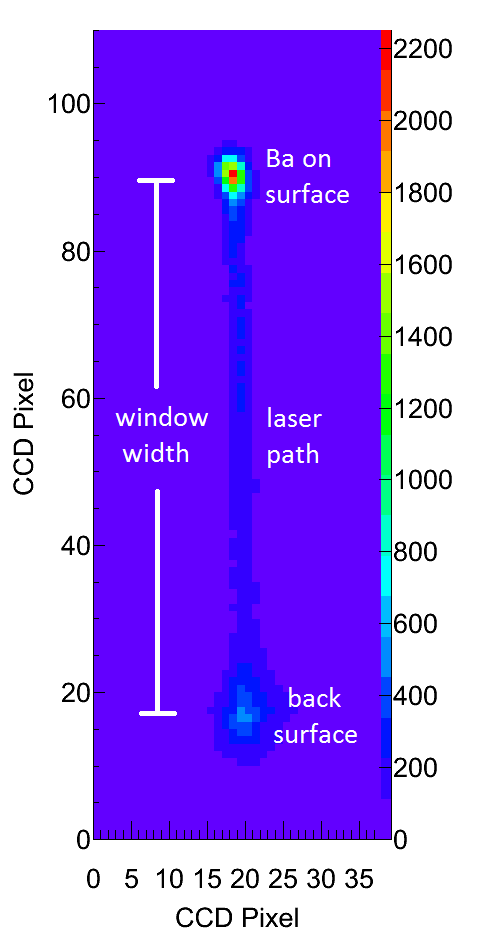
\includegraphics[width=0.35\textwidth]{figures/raw_14-atom_labels_from_paper_1f.png}
  %\end{center}
  %\caption{}
  %\label{fig:imageexamp}
%\end{wrapfigure}

\section{Imaging 577- and 591-nm Fluorescence}
\label{sec:imaging590and577}

\begin{figure} %[H]
        \centering
                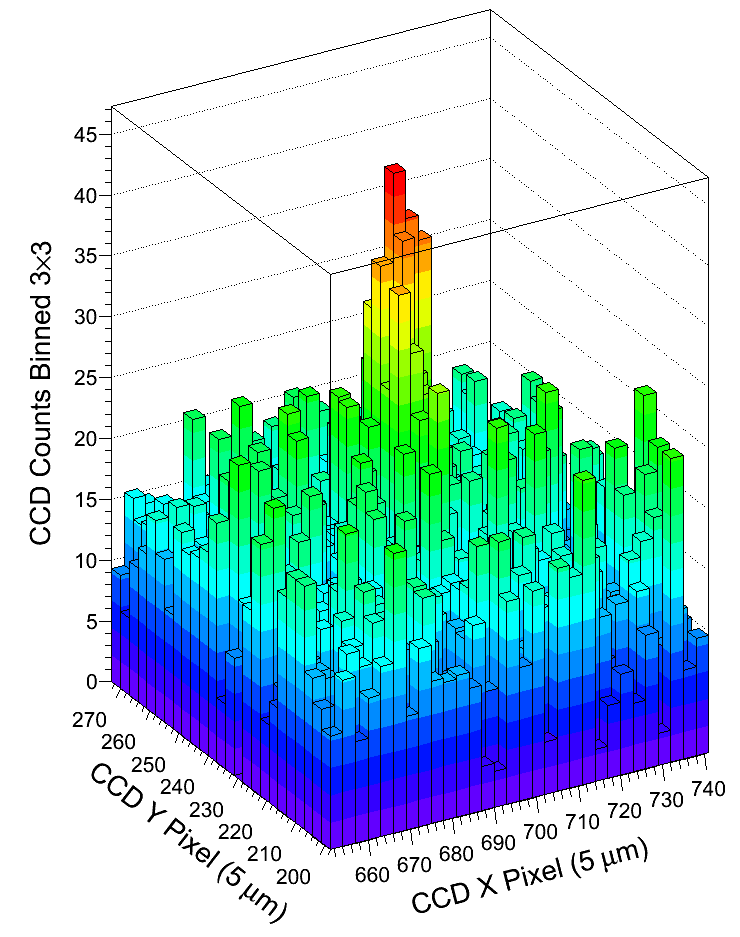
\includegraphics[width=.6\textwidth]{figures/image_1e4.png}
                \caption{Image through 586-nm band-pass filter of $\leq 2.7 \times 10^{3}$ average Ba atoms in SXe.  100-s exposure with .03~$\mu$W of 566~nm excitation, with laser beam waist of 5~$\mu$m.  Sample was deposited at 50~K and observed at 11~K.  $3 \times 3$ pixel binning was done with software.}
\label{fig:image590s}
\end{figure}

First attempts at imaging small numbers of Ba atoms in a focused laser region were done with the 577- and 591-nm Ba fluorescence peaks together using a 586-nm band-pass filter, which passes 573 - 599~nm FWHM.  This filter has a 2" diameter, resulting in a collection efficiency of $8.4 \times 10^{-3}$, 4$\times$ the efficiency given in Table \ref{table:colleff}.  An image of $\leq 2.7 \times 10^{3}$ atoms on average, with $\leq 8.3 \times 10^{3}$ total atoms exposed, is shown in Fig. \ref{fig:image590s} for a 100-s exposure with 0.02~$\mu$W of 566-nm excitation.  The laser was focused by the bi-convex lens, resulting in a beam waist of 5~$\mu$m as discussed in Sec. \ref{sec:laser}.  With this spot size, the factor between total and average atoms exposed is 3, as discussed in Sec. \ref{sec:vibes}.  At this low intensity, no bleaching was observed in the four frames observed (frame 1 is shown).  Groups of 9 ($3 \times 3$) CCD pixels have been binned in software to produce the nice peak shown.  As discussed in \ref{sec:bleaching}, detection of very small numbers of atoms in these sites may require several re-pump lasers.  As a result of low total exposure, neither the sapphire nor the surface backgrounds are present in these images, though a Xe-only image has been subtracted. 

%$5 \times 10^{3}$        $\leq$ 10$^{4}$

%(10$^{4}$ Ba\textsuperscript{+} ions deposited into the effective laser region)

%Bleaching data was used to optimize laser intensity and exposure time to achieve maximal signal in frame 1, and to avoid hole bleaching.  The fast bleaching of these peaks is the limiting factor on sensitivity.

\begin{figure} %[H]
        \centering
                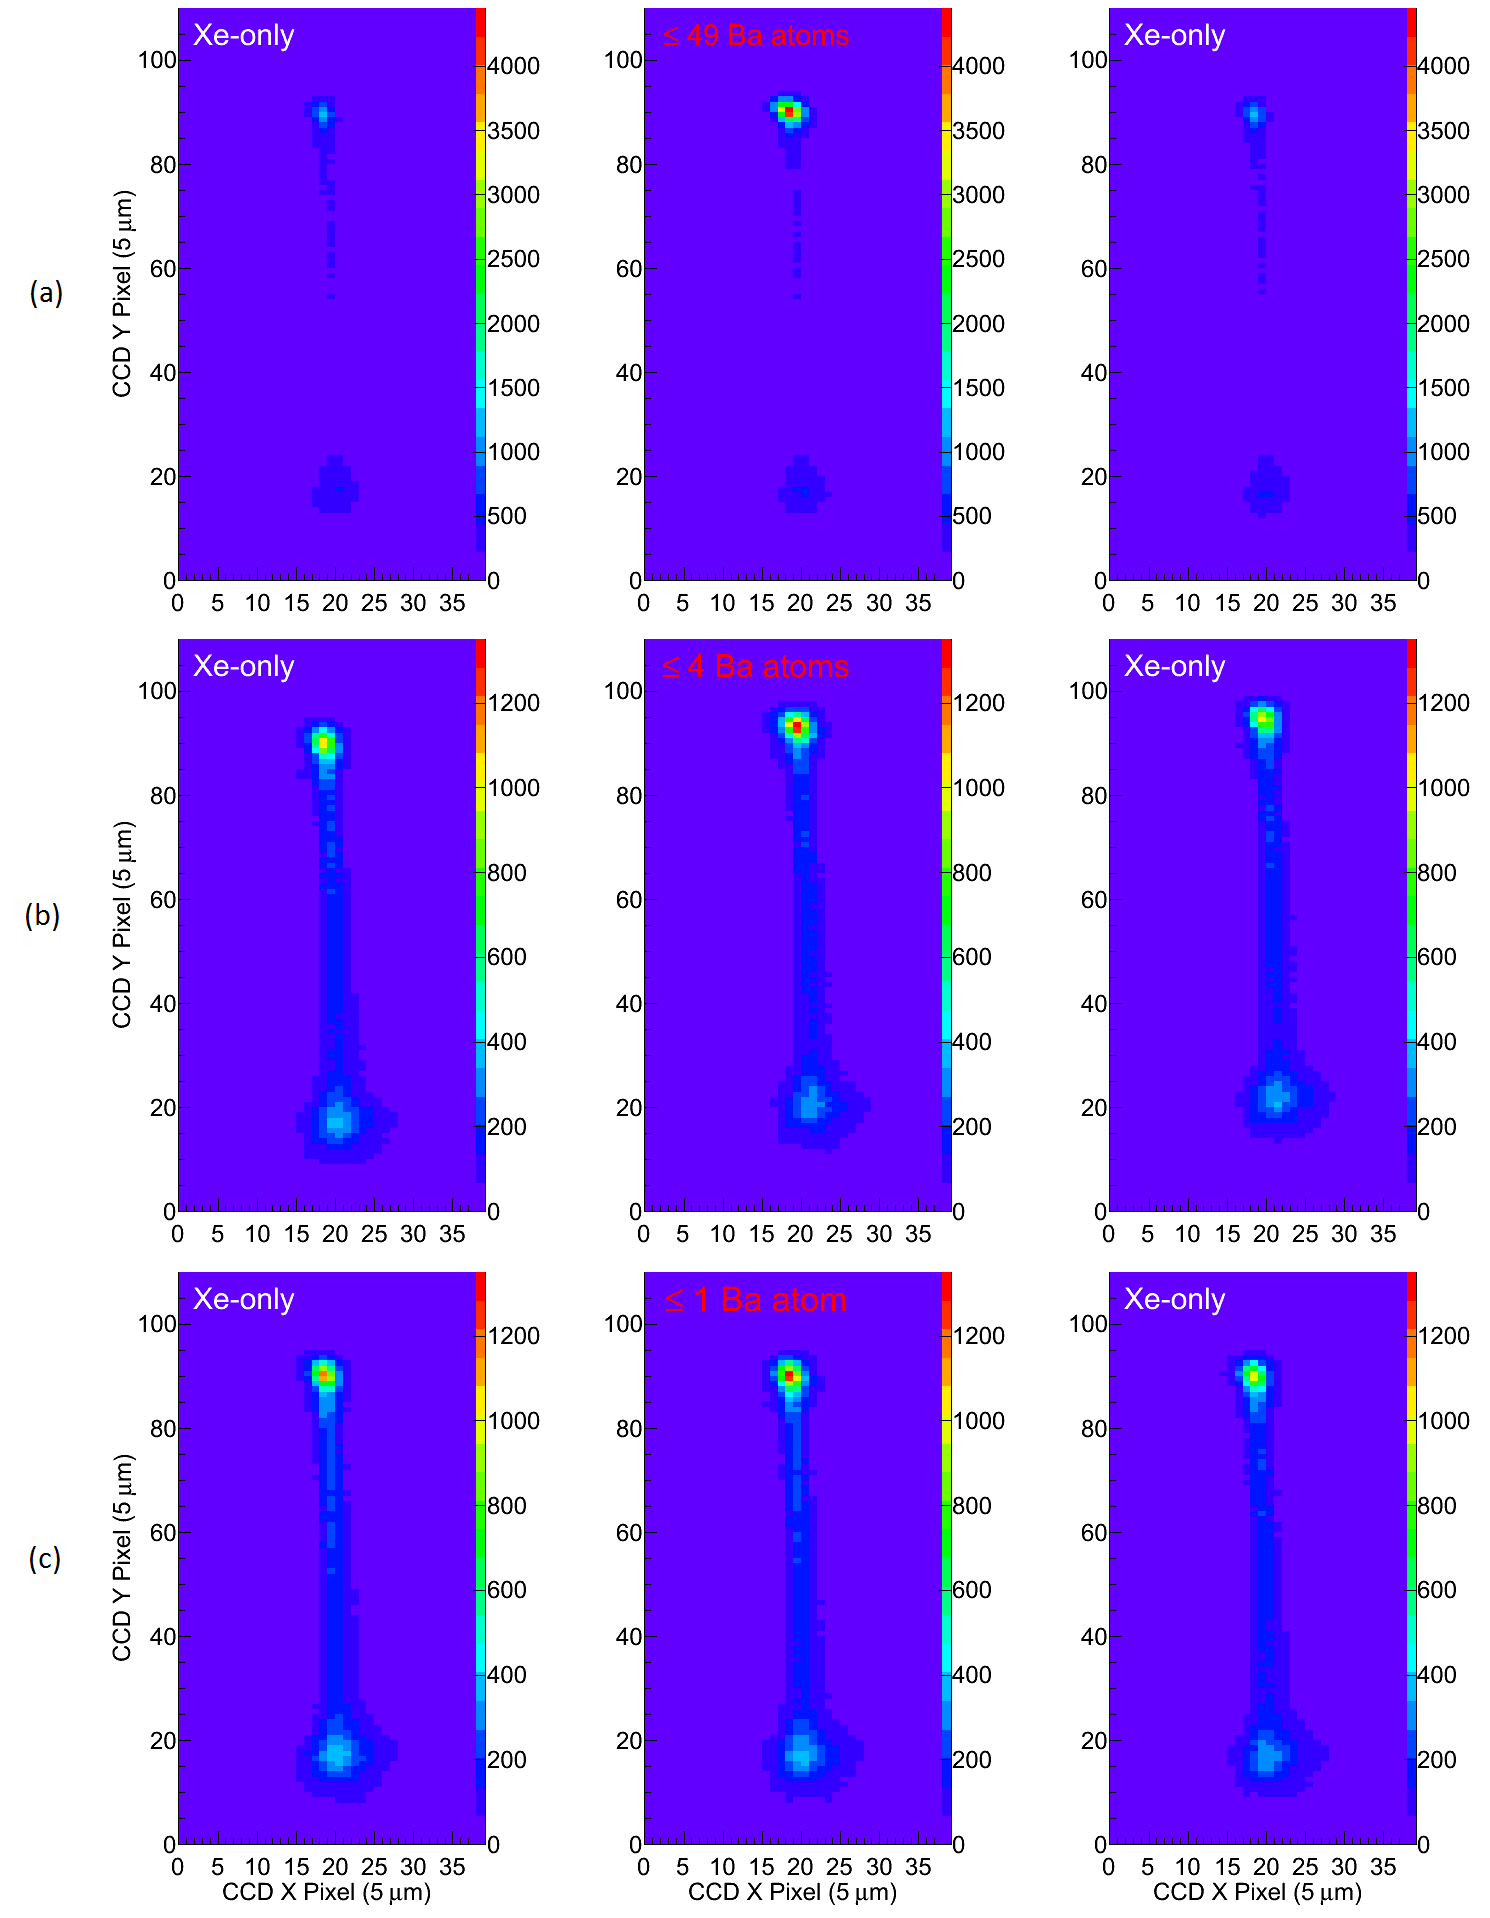
\includegraphics[width=.95\textwidth]{figures/xebaxe_average_scrunched.png}
                \caption{\emph{\color{gray}change Ba text to likeo range instead of red -- it doesn't even show up well in color} Raw images through 620-nm band-pass filter of three Ba\textsuperscript{+} deposits yielding (a) $\leq 49$, (b) $\leq 4$, and (c) $\leq 1$ average number of Ba atoms, with their preceding and succeeding Xe-only deposits.  Samples were deposited at 50~K and observed at 11~K.  Exposures are 60~s with around 0.24~mW of 570~nm excitation focused to w$_{\text{x}} \times$ w$_{\text{y}} =$ 2.06~$\mu$m $\times$ 2.66~$\mu$m.}
\label{fig:xebaxe}
\end{figure}

\section{Imaging 619-nm Fluorescence}
\label{sec:imaging619}

Raw images of Ba\textsuperscript{+} deposits and their preceding and succeeding Xe-only deposits are shown in Fig. \ref{fig:xebaxe} for deposits of (a) $\leq 49$ ($\leq 230$), (b) $\leq 4$ ($\leq 20$), and (c) $\leq 1$ ($\leq 5$) average (total) Ba atoms.  The aspherical laser focusing lens and astigmatism compensator were used for a w$_{\text{x}} \times$ w$_{\text{y}} =$ 2.06~$\mu$m $\times$ 2.66~$\mu$m 1/e$^{2}$ laser region, and thus the factor between total and average atoms exposed is 4.7.  Signal is distinguishable from background by eye, even at the 1-atom average signal level.

%An imaging experiment consisted of many different pulsed Ba\textsuperscript{+} deposits, each of which was evaporated after observation.  This procedure is described in \ref{sec:deposition}-\ref{sec:collection}.

\begin{figure} %[H]
        \centering
                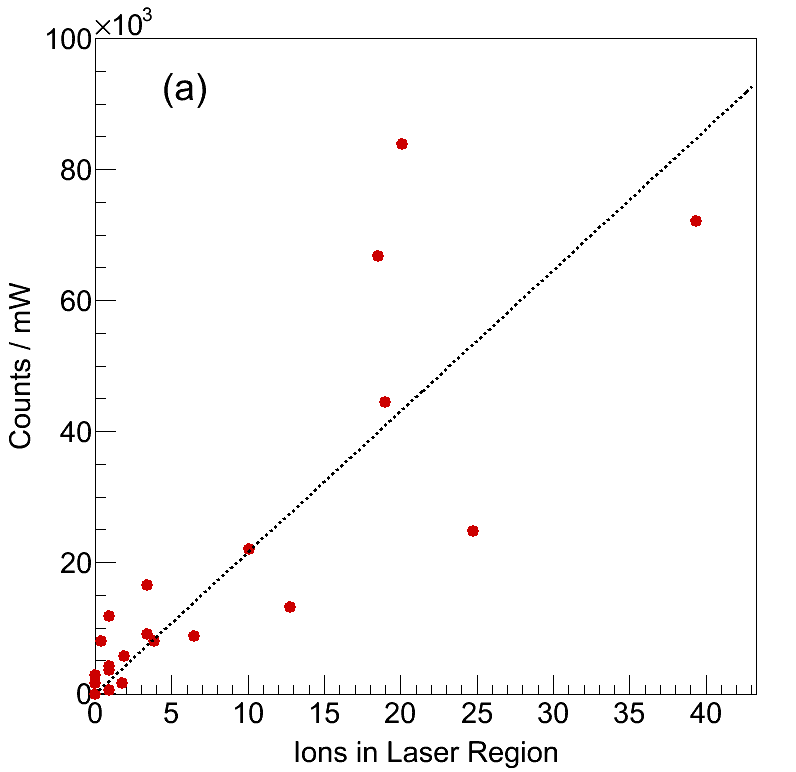
\includegraphics[width=.5\textwidth]{figures/lin_just20150807_lin.png}
                ~
                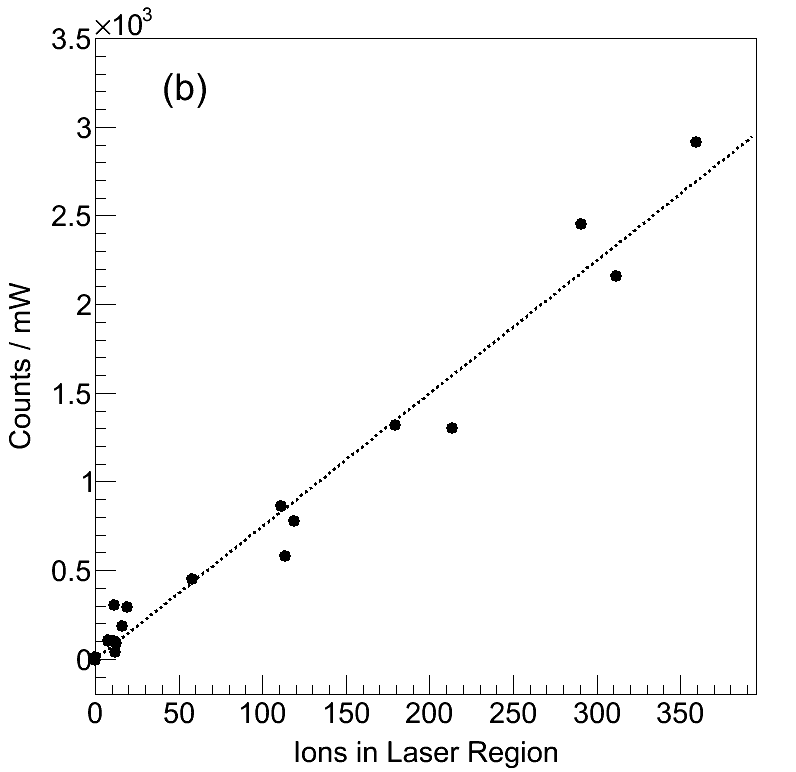
\includegraphics[width=.5\textwidth]{figures/lin_just20150526_lin.png}
                \caption{619-nm signal, scaled by laser power, vs. average number of Ba\textsuperscript{+} exposed by focused laser at 570~nm for experiments with (a) aspherical, and (b) bi-convex laser focusing lenses.  Exposure times are (a) 60~s, and (b) 3~s.}
\label{fig:lin}
\end{figure}

\begin{figure} %[H]
        \centering
                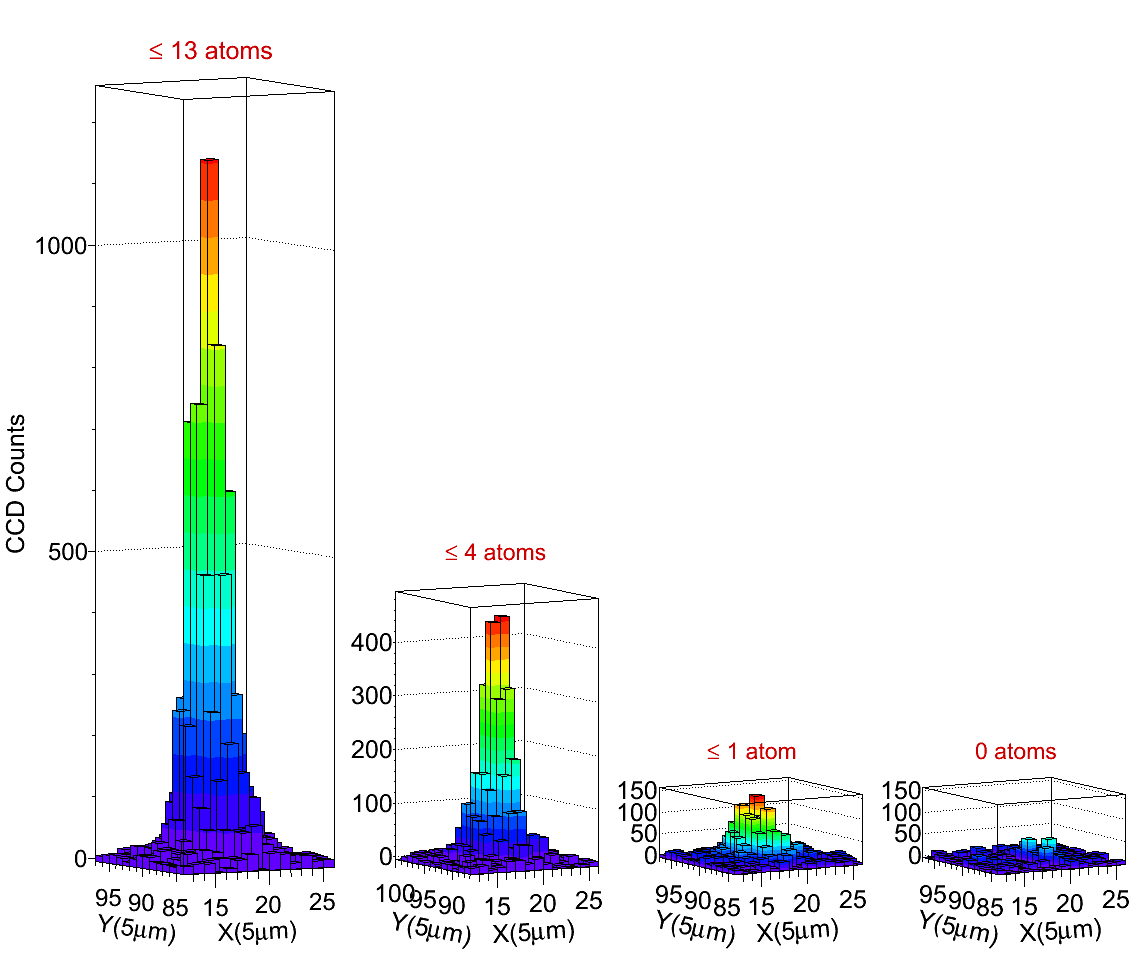
\includegraphics[width=.99\textwidth]{figures/train.png}
                \caption{Subtracted images of 619-nm fluorescence in focused laser region for runs near linear trend line in signal vs. ions deposited.  Exposures are 60~s with around 0.24~mW of 570~nm excitation focused to w$_{\text{x}} \times$ w$_{\text{y}} =$ 2.06~$\mu$m $\times$ 2.66~$\mu$m.}
\label{fig:train}
\end{figure}

619-nm fluorescence signal is plotted vs. average number of ions (upper limit on atoms) exposed in Fig. \ref{fig:lin} for many deposits in two experiments with two different laser focusing lenses.  The aspherical lens with astigmatism compensation (a) results in w$_{\text{x}} \times$ w$_{\text{y}} =$ 2.06~$\mu$m $\times$ 2.66~$\mu$m, while the bi-convex laser-focusing lens with no astigmatism compensation (b) results in a laser waist of $w = 5~\mu$m.  Exposures were (a) 60~s with 0.24~mW laser power, and (b) 3~s with 2~mW laser power.  The signal was determined by summing the counts of a 3-pixel$\times$3-pixel (15$\mu$m$\times$15$\mu$m) region centered on the laser spot in the image, and background was determined by averaging the 3-pixel$\times$3-pixel sum of the Xe-only runs before and after each Ba\textsuperscript{+} run.  Signal and background were scaled to laser power, and then background was subtracted.  The two experiments demonstrate linear relationships between signal and number of ions exposed over more than two orders of magnitude.  Zero ion deposits are produced by retracting the Faraday cup for 1~s without pulsing the ion beam.  The slope of the linear fit in (a), which does not include a constant value, gives about $1500 \pm 160$~counts/mW per atom with 60-s exposures.  Deposits at the single-ion level average to $5000 \pm 2400$~counts/mW.
%, somewhat higher than the linear trend line.

Images of 619-nm Ba fluorescence are shown in Fig. \ref{fig:train} for a few deposits near the linear trend line.  Each has subtracted an image of a nearby Xe-only deposit so that only the Ba fluorescence is seen.  Clear, sharp peaks are observed from an average number of atoms all the way down to the single-atom level, with no clear peak in the zero-atom deposit.  This result is a major step toward the ultimate success of Ba tagging, and is generating excitement and interest in the nEXO collaboration.

\begin{figure} %[H]
        \centering
                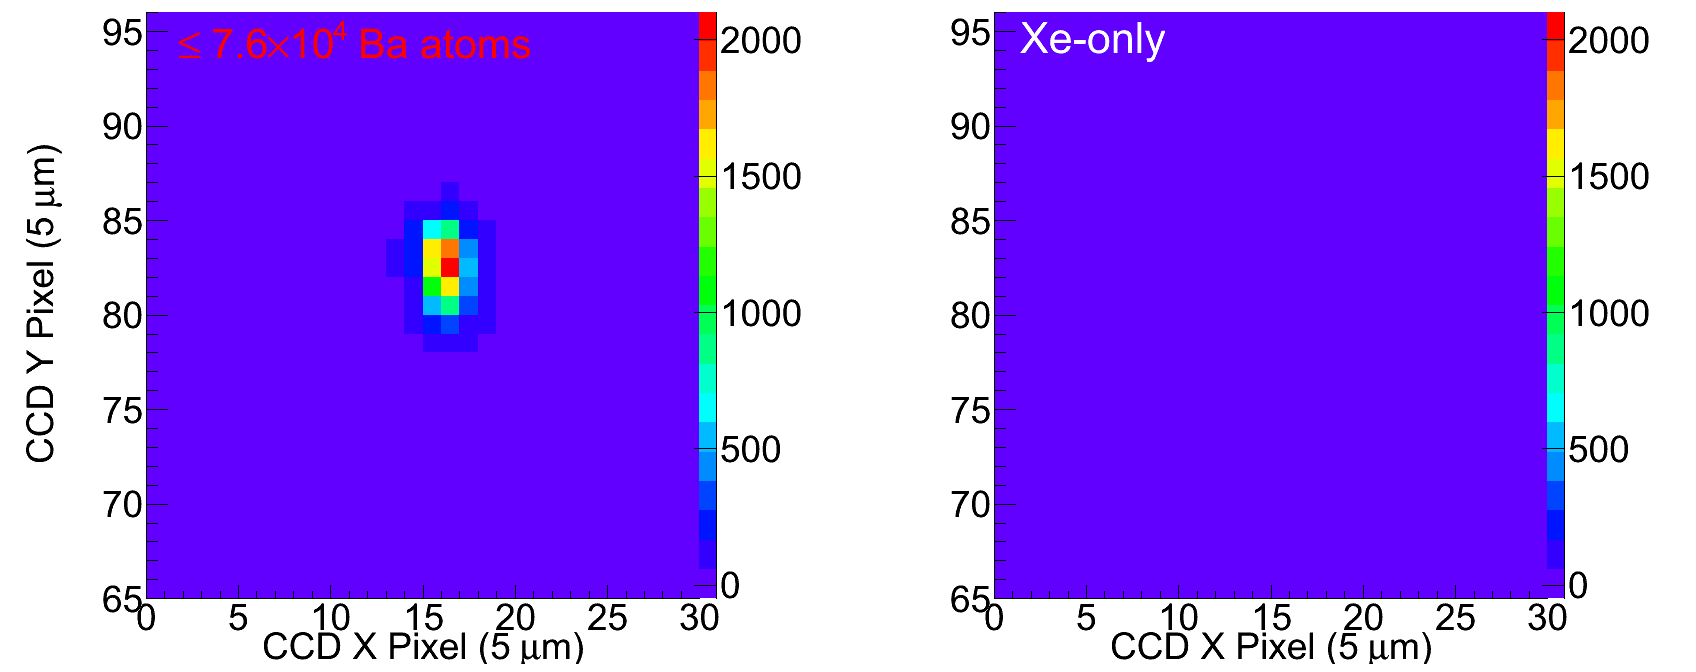
\includegraphics[width=.95\textwidth]{figures/xebaxe_largest_average.png}
                \caption{\emph{\color{gray}change Ba text to likeo range instead of red -- it doesn't even show up well in color} Raw images through 620-nm band-pass filter of a Ba\textsuperscript{+} deposit yielding $\leq 7.6 \times 10^{4}$ average number of Ba atoms, with its preceding and succeeding Xe-only deposits.  Exposures are 0.5~s with 0.6~mW of 572~nm excitation focused with asphere and astigmatism compensator.}
\label{fig:xebaxeLarger}
\end{figure}

Another important observation is the lack of historical buildup of Ba fluorescence between deposits, even for large Ba\textsuperscript{+} deposits.  This is demonstrated in Fig. \ref{fig:xebaxe}, where the Ba fluorescence is no longer present in the Xe-only runs following each of the deposits.  This is shown further for a deposit 10$\times$ larger in Fig. \ref{fig:xebaxeLarger}.  The stronger presence of laser path through the sapphire window is caused by higher Cr\textsuperscript{3+} content in the window used in this experiment.  The disappearance of Ba signal after evaporation of each sample is important for the implementation of this method of Ba tagging on a probe in nEXO.

\section{Scanned Images}
\label{sec:scanning}

The ultimate demonstration of single-atom imaging will be to scan the focused laser over samples with more widely separated Ba atoms, observing a peak when the laser moves over individual atoms.  The resolution in a scanned image is determined by the laser spot size, even when the imaging optics have a lower resolution.  Preliminary scans were performed by scanning the focusing lens in a raster pattern, using the setup described in Sec. \ref{sec:laserscanning}.  Summed counts/mW from a $3 \times 3$ pixel area around the focused laser are plotted vs. raster position for several deposits in Fig. \ref{fig:scans}.  These scans are grids of 20 points in X at about 3.75~$\mu$m/step, by 5 points in Y at about 4.78~$\mu$m/step.  An overall higher signal is observed with 48.4 average Ba\textsuperscript{+}/step (c), however single-atom peaks are not distinguished in the sparse deposit of 0.18 average Ba\textsuperscript{+}/step (b).  The aspherical laser focusing lens and astigmatism compensator are used for w$_{\text{x}} \times$ w$_{\text{y}} =$ 2.06~$\mu$m $\times$ 2.66~$\mu$m 1/e$^{2}$ laser region, though cryostat vibrations increase the exposed region as described in Sec. \ref{sec:vibes}.  This had the effect of exposing neighboring step regions to the laser.  Pre-bleaching of the surface background was done with a raster of the dye laser at 580.5~nm, in a $22 \times 7$ grid centered on the $20 \times 5$ grid used during the following experiment, with 10~s at each location.

\begin{figure} %[H]
        \centering
                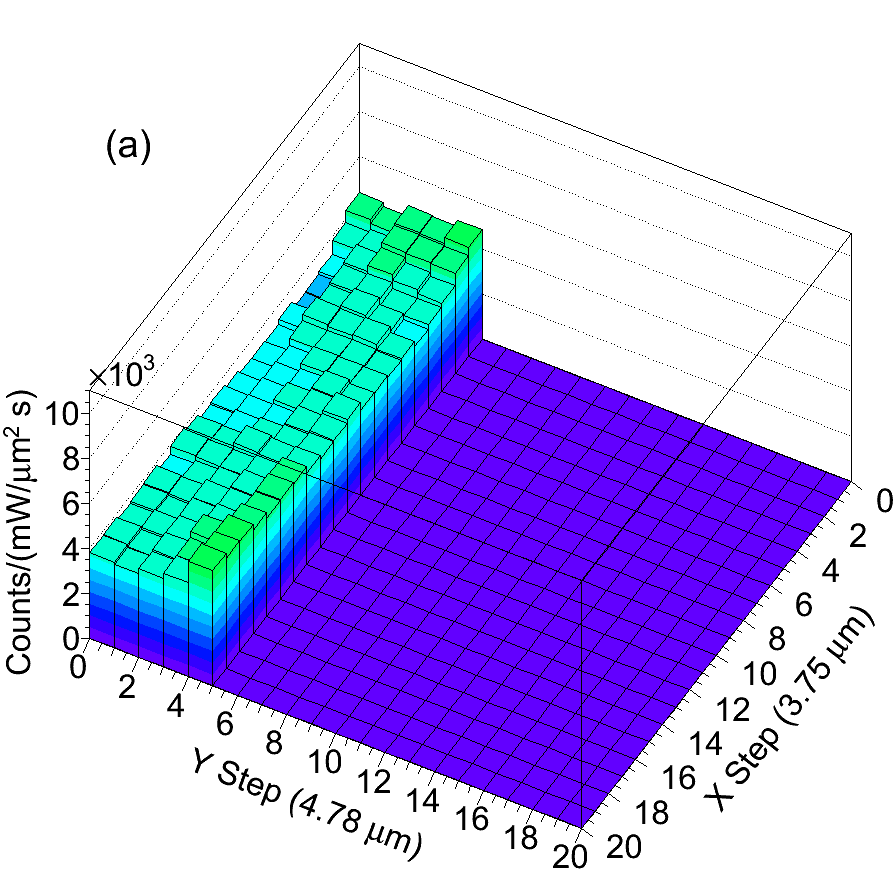
\includegraphics[width=.5\textwidth]{figures/scan_a.png}
                ~
                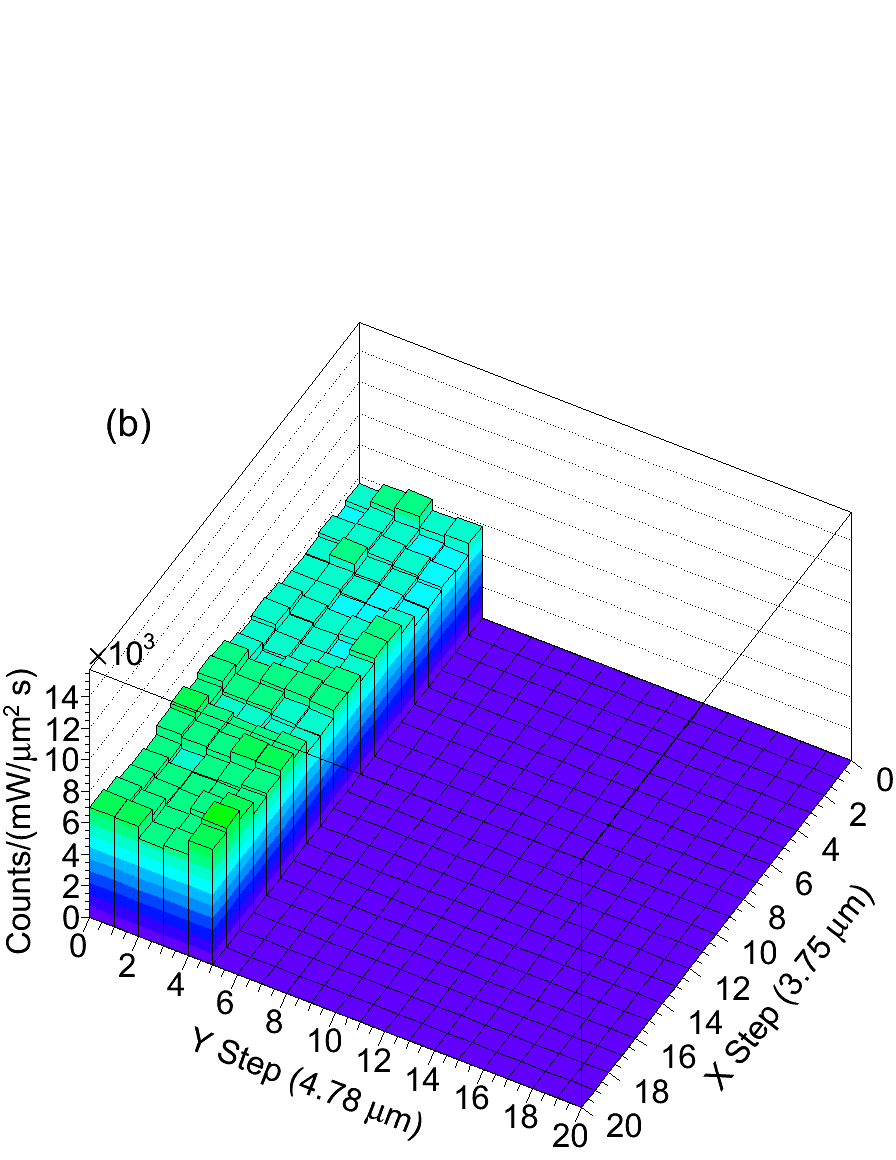
\includegraphics[width=.5\textwidth]{figures/scan_b.png}
                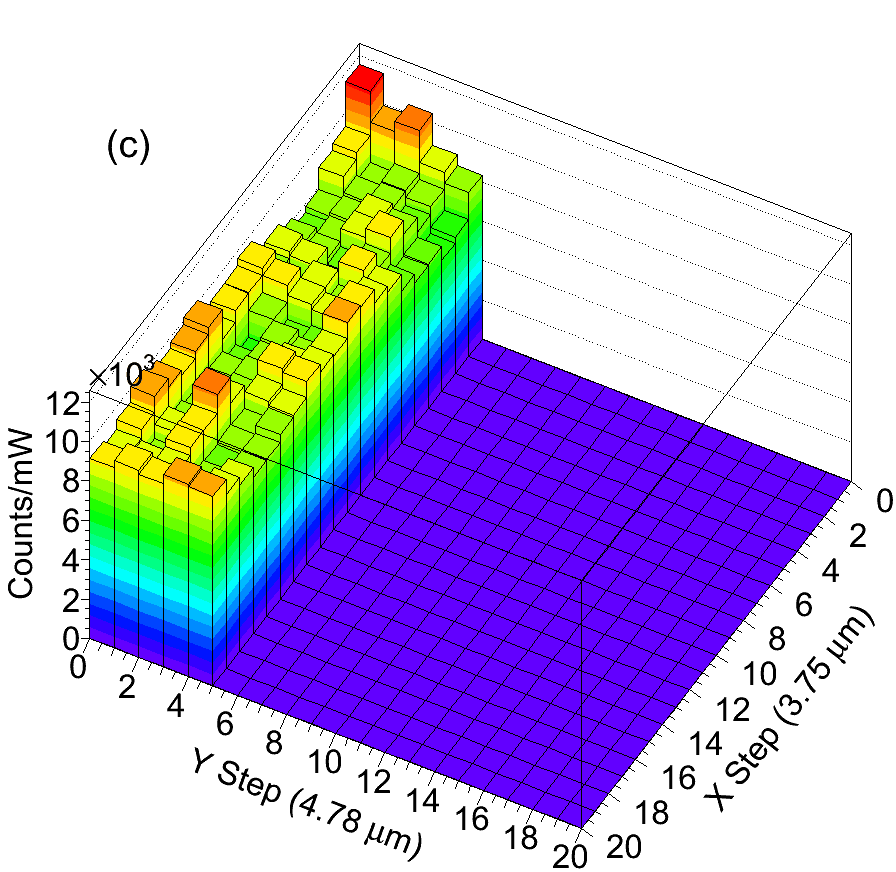
\includegraphics[width=.5\textwidth]{figures/scan_c.png}
%                ~
%                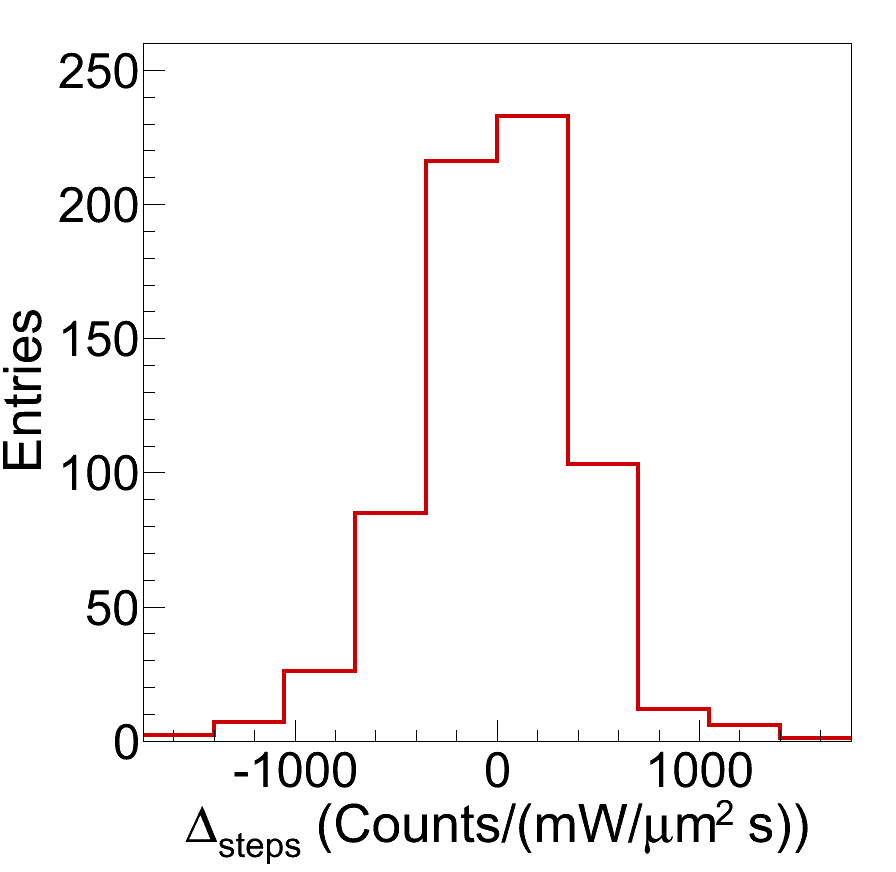
\includegraphics[width=.5\textwidth]{figures/scans_dframeXe.png}
%                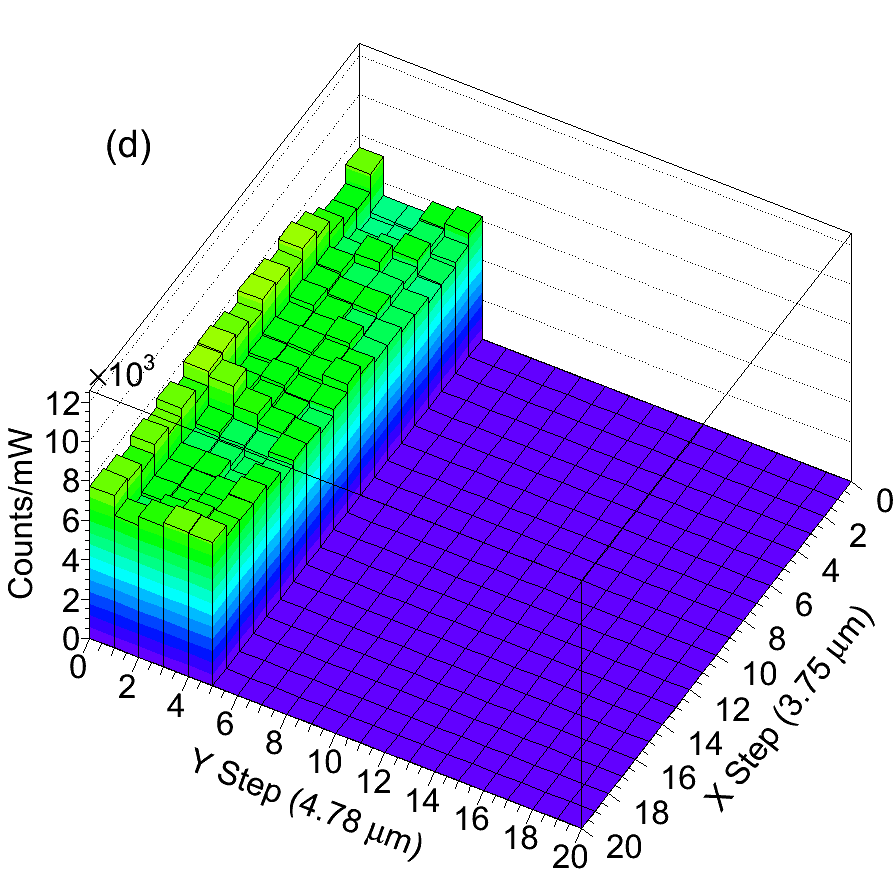
\includegraphics[width=.5\textwidth]{figures/scan_d.png}
%                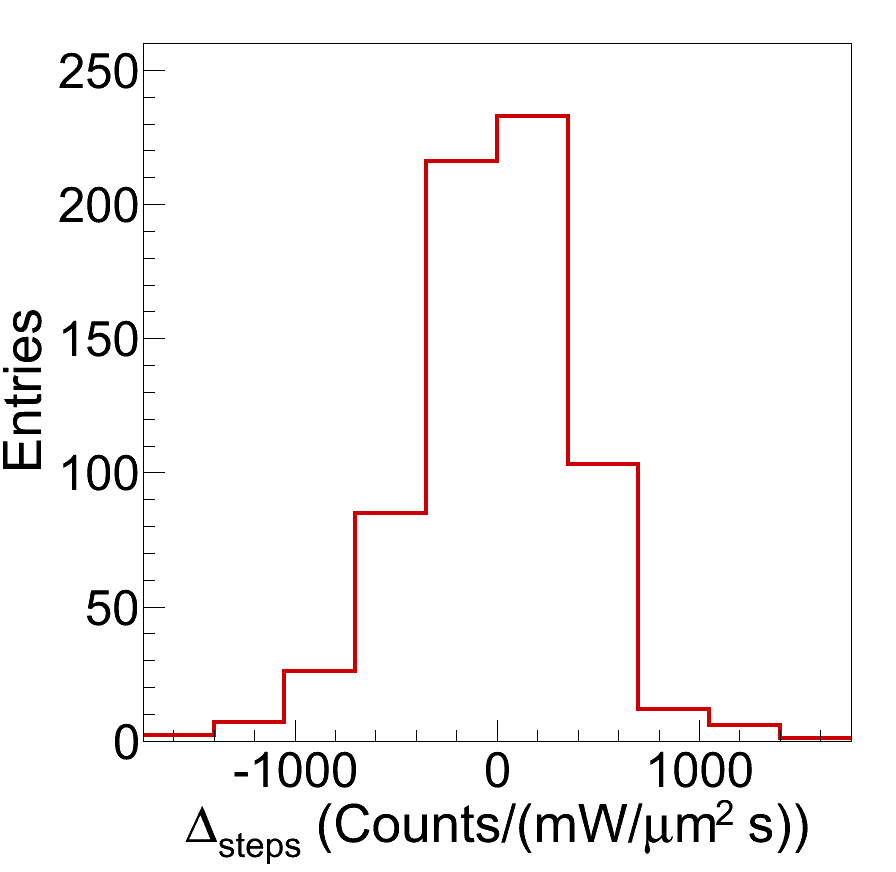
\includegraphics[width=.45\textwidth]{figures/scans_dframeXe.png}
                \caption{\emph{\color{gray}change to show the 6 Ba per, since the counts number is from that, and also show the one with the solid single atom peak, heh...}Early attempts at scanned images of a few deposits: (a) Xe-only, (b) 0.18 average Ba\textsuperscript{+}/step, and (c) 48.4 average Ba\textsuperscript{+}/step.  Exposures are 10-s with 0.4-0.5~mW of focused 570~nm laser.}
\label{fig:scans}
\end{figure}
%, and (d) Xe-only

\begin{figure} %[H]
        \centering
                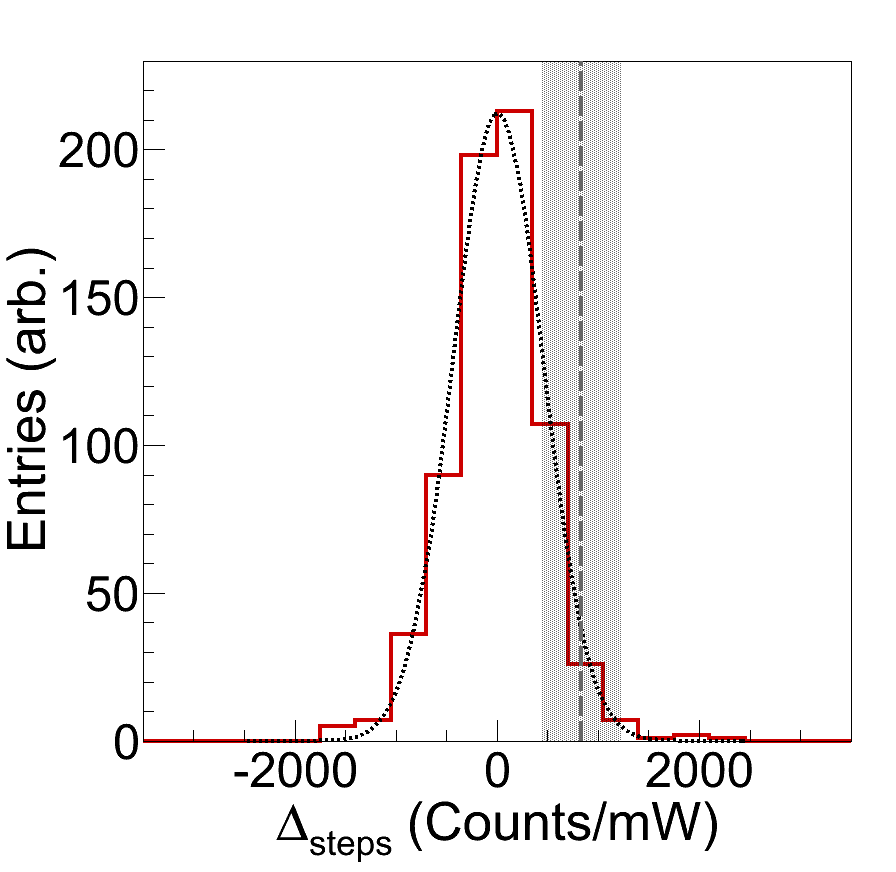
\includegraphics[width=.5\textwidth]{figures/xevar_scanDelta.png}
                ~
                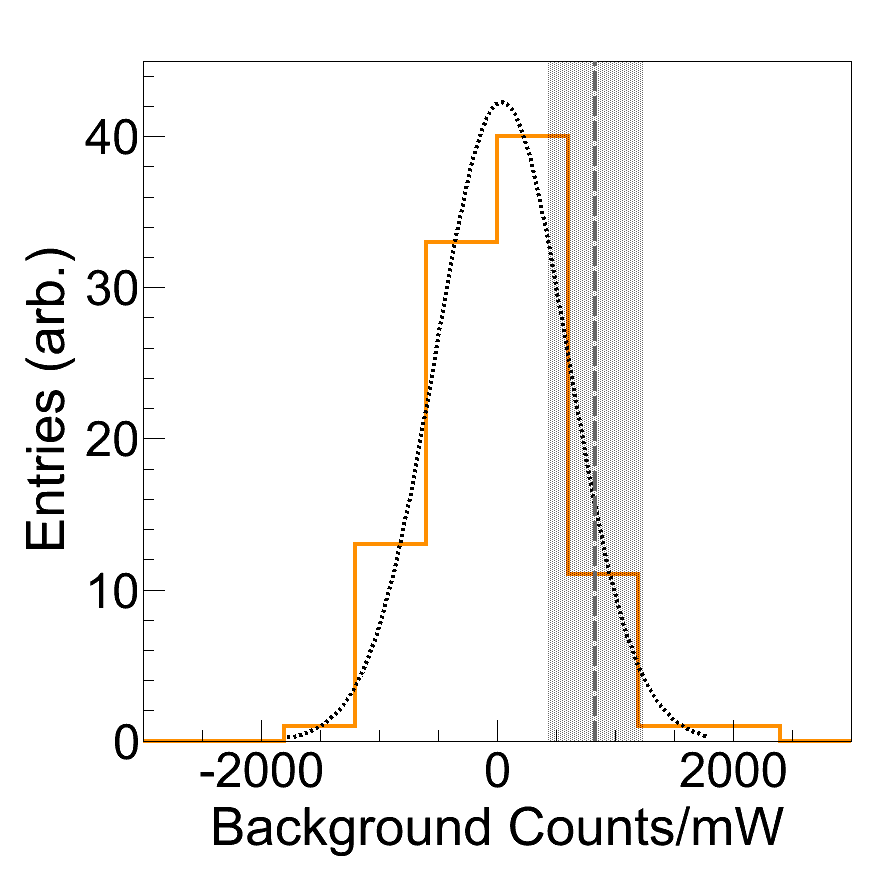
\includegraphics[width=.5\textwidth]{figures/xevar_scanSubtraction.png}
                \caption{\emph{\color{gray}change (b) to ste-to-tep rather than just straight dist.}  Distribution of difference in counts ($\Delta_{\text{steps}}$) between successive scan frames in (a) raw Xe-only deposits, and (b) the subtraction of two Xe-only runs.}
\label{fig:scanVarXe}
\end{figure}

Signal and background levels from the scanned images in Fig. \ref{fig:scans} are consistent with previous experiments, with approximately 440~counts/mW {\color{red}$pm$ ???} per Ba atom, and about 4500~counts/mW background, with 10-s exposures.  However, the scanned images of Xe-only deposits (Fig. \ref{fig:scans}(a)) produce a measure of step-to-step variation in the surface background which competes with the single-atom signal level for about {\color{red}? -- get from the $\sigma$ value}\% of the fluctuations.  The difference in counts between successive grid steps is shown as a distribution in Fig.\ref{fig:scanVarXe}(a) for all Xe-only deposits in this set of scanned images.  The single-atom signal level of {\color{red}$833 \pm ???$}~counts/mW (for 10-s exposure) is marked with a gray dotted line, which intersects the background distribution at the ? level.  The step-to-step variation in the subtraction of two Xe-only scanned images is shown in Fig. \ref{fig:scanVarXe}.  This distribution is somewhat broader than that of the raw background images, with the single-atom level intersecting at the ? level.  It is difficult to distinguish single Ba atoms from background fluctuations under these conditions.

Since the single-atom signal level of {\color{red}$833 \pm ???$}~counts/mW assumes 100\% conversion of deposited Ba\textsuperscript{+} ions, it is possible that single Ba atoms produce more signal than this.  Thus, it is possible that, e.g., the peak around (?,?) in Fig. \ref{fig:scans}(?) is due to a single atom.  However, background levels must be reduced further to be sure.  The next steps in scanned imaging of Ba atoms, discussed in Sec. \ref{sec:future}, will involve reducing the surface background.

%\emph{\color{gray}choose what to show and what to say about it -- there are some decent things to show really}  [issues are BG, reproduceability, vibrations]

%\emph{\color{gray}See thought\_process.pptx slide about expected signal / observed BG fluctuation, etc. (unfinished).}